\section{Practical Lightweight Nondeterminism
  Detection and Debugging}

\begin{figure}
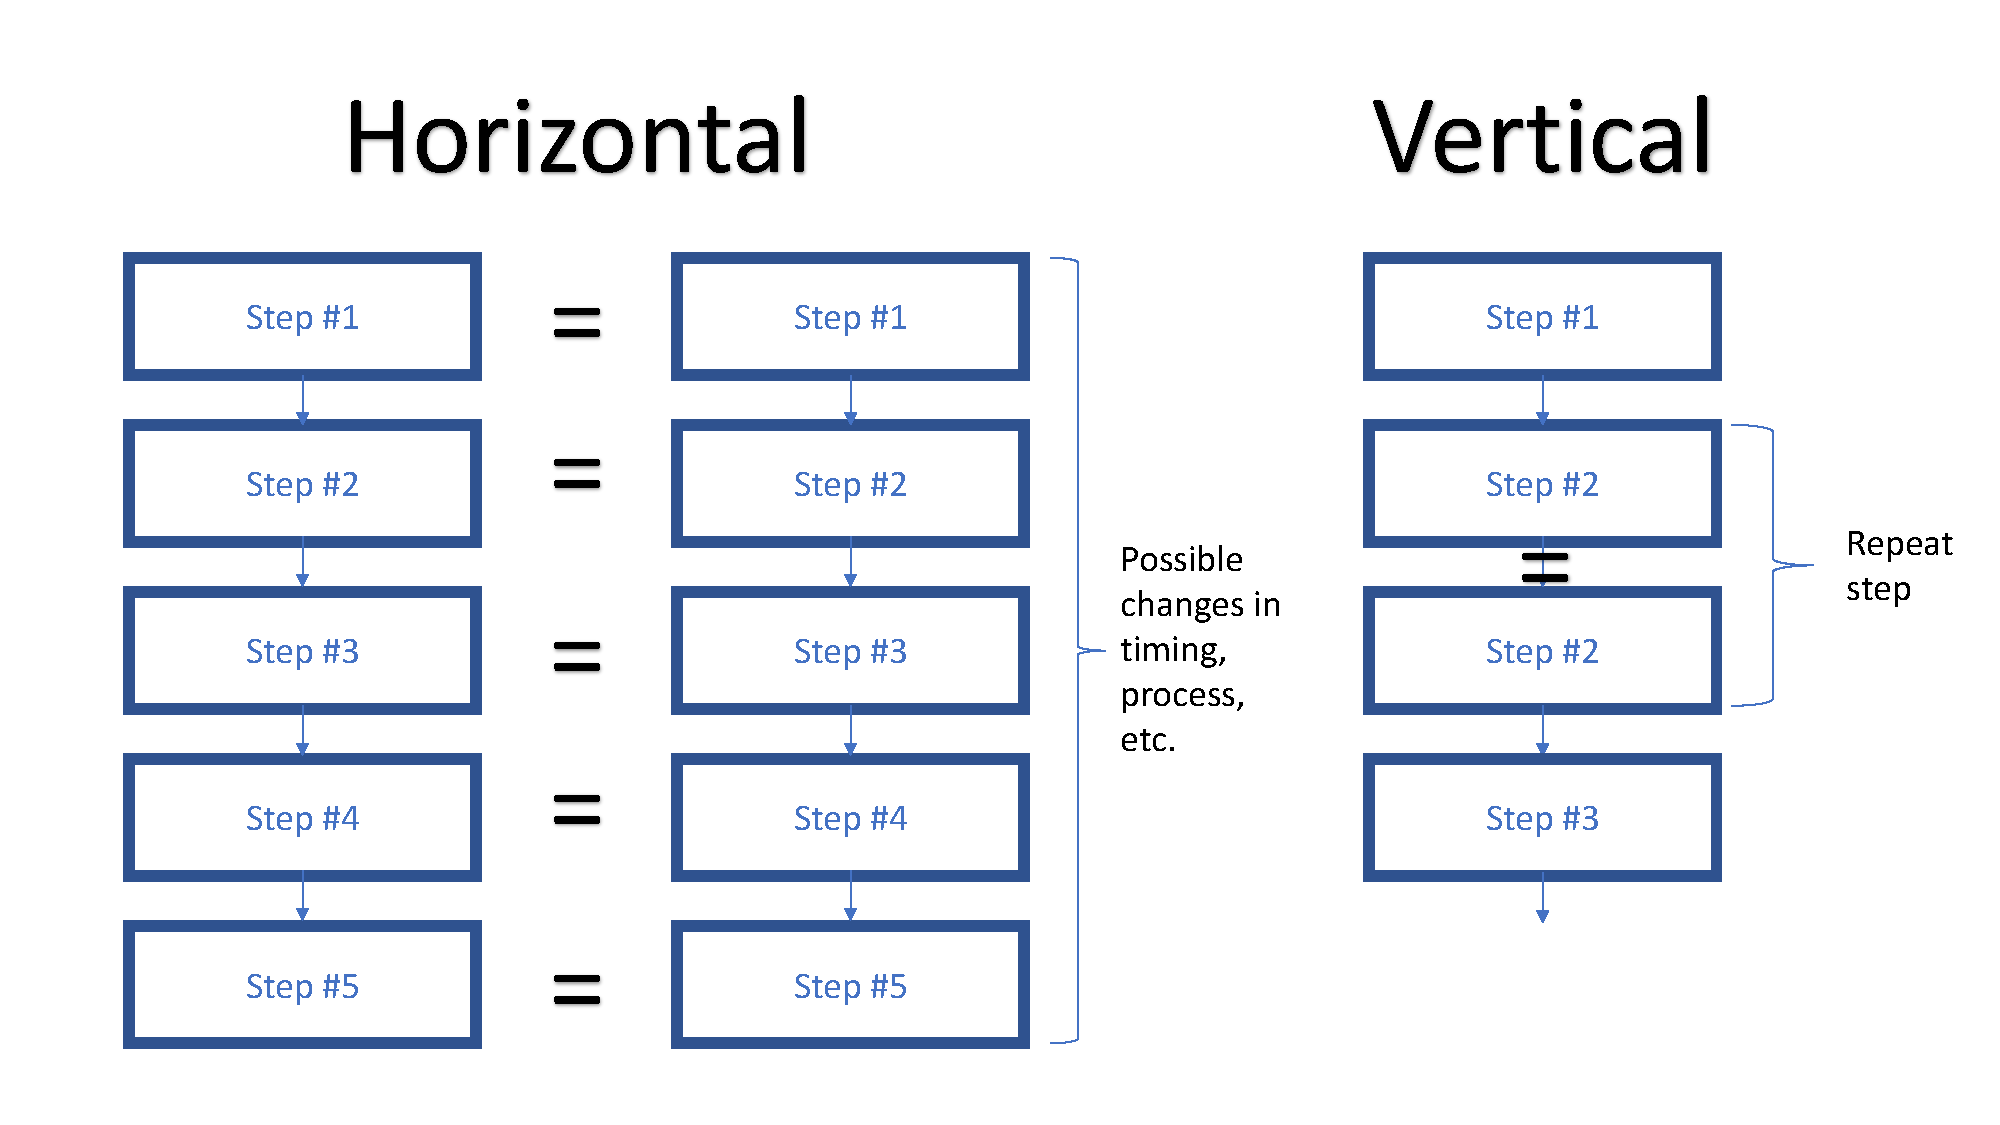
\includegraphics[width=\columnwidth]{types}
\caption{Types of determinism}
\label{fig:types}
\end{figure}

We define two basic types of determinism, shown in Figure
\ref{fig:types}:  horizontal determinism and vertical determinism.  In
horizontal determinism, which is what we usually think of when we
think about deterministic behavior, a software system reliably
produces the same behavior given the same steps of a test: the
behavior of multiple executions that are ``the same'' in terms of
inputs/actions can be aligned and checked for some type of equality.  In
vertical determinism, rather than behavior across executions, we are
interested in behavior within an execution, where repeating the same
step of a test twice should result in the same behavior.  Obviously,
vertical determinism is both rarer and more specialized than
horizontal determinism.  However, in those instances, vertical
determinism is arguably more important than horizontal determinism, in
that violations usually indicate a potentially serious fault.

\subsection{Horizontal Determinism}


\subsubsection{Determinism and Reflexive Differential Testing}

Horizontal determinism can be best understood by thinking of
nondeterminism detection as an unusual kind of \emph{differential
  testing} \cite{Differential,ICSEDiff}.  In differential testing, a
system is compared against a reference in order to ensure that
it behaves equivalently, at some level of abstraction, to another
implementation of the same functionality.  Differential testing is
extremely powerful, in that any divergence of behavior, if divergence
is correctly defined, indicates a functional correctness fault in (at
least) one of the systems under test.  Being able to detect functional
correctness errors without the cost of constructing a formal
specification is extremely useful in automated test generation.  Differential testing is widely
used for systems software components such as compilers
\cite{Differential,csmith} and POSIX file systems \cite{CFV08,AMAI}, where multiple
implementations are common.  The major limitation of differential
testing, of course, is that multiple implementations of a system are
almost as rare as good correctness specifications.

For the special case of detecting nondeterminism, however, \emph{a
  system can serve as its own reference implementation.}    The
question, then, becomes one of deciding at what granularity the
reference equivalence will be checked:  as discussed above,
processor-instruction and memory-layout determinism is seldom
necessary or even desired (it would greatly limit optimizations of
code execution).  We propose two approaches to ``aligning'' an
execution with itself.

\subsubsection{Visible Value Determinism}

Visible value determinism uses the human-accessible outputs (displayed
or stored to a file), and \emph{values returned by functions or methods
called as a library by other code}, as the criteria for determining if two executions
are equivalent.  The idea is simple:  determinism is motivated by the
desire to create consistent behavior for an observer, whether that
observer is a human user, another software system, or a regression
test.  The values output by a software element are the only values of
interest to the observer.  In practice, of course, some values (time
stamps, pointer addresses, etc.) are not expected to be deterministic
by an observer; we call these values \emph{opaque} in that they are
not interpretable as ``showing'' the internal workings of the code
being tested for determinism.  Rather, they mask an abstraction,
usually one managed by the operating system (system
time, memory management).   Any mechanism for visible value
determinism needs to support automatic and manual designation of some
values as opaque.

\subsubsection{Final State Determinism}

Visible value determinism has significant limitations.  While it
provides the finest granularity for detecting nondeterminism, which is
important for debugging purposes, it is also expensive, requiring
checks on (and possibly storage of) a potentially very large number of
values.  Additionally, in some cases so many values produced by a
system are opaque that the annotation burden is inordinate.  In these
cases, it is better to only compare final states of a computation
performed by the system being checked for determinism.  The final
state may have opaque components, but it is easy to define an
abstraction that reduces the state to the actual value of interest.


%\subsubsection{Core Sources of Difference:  Timing and Process}

\subsection{Vertical Determinism}

Vertical determinism is a property that expresses that some operations
of a software system should, within the same trace, always behave the
same way.  Usually, for interesting cases, this is dependent on some
state of the system, though some operations should be completely
state-independent.  E.g, the hash of a given bytestring returned by a
security library should never change.  This is one aspect of
\emph{pure} functions.  For nondeterminism checking, the interesting
cases are non-pure: a function depends on system state, but should
always depend on it in the same way, and should not, itself, change
system state in a way that would change its behavior on a subsequent
run.

Many \emph{idempotent} operations fall into this category.
Consider adding an element to an AVL tree implementing a set, not a
multiset.  Assume the method call returns the parent node of the
element, whether it was added or was already in the tree.  Calling
this method any number of times in sequence should always return the
same value, though the first call may have modified the contents of
the AVL tree.

One application of vertical determinism, then, is to identify
idempotent operations in an automated test generation harness, and
simply automatically retry all such operations, checking that the
result is unchanged.  The overhead of vertical nondeterminism detection will
generally be much lower than that for horizontal nondeterminism
(horizontal checks must re-execute an entire test; vertical checks
only re-execute proportional to the number of idempotent operations
performed).  However, identifying idempotent operations is a
fairly serious specification burden.  Are there instances where a tool
can automatically identify a limited kind of idempotent behavior?

\subsubsection{Failure Determinism}

A specialized case of vertical determinism is failure determinism.
Failure determinism is the following restriction on an API:

{\bf If a call fails, and indicates this to the caller, it should not modify system
  state in any way.  Changes made before the failure should be rolled
  back.} 

In other words, failure determinism is a property stating that an API
is \emph{transactional} with respect to failures (it may not be so
with respect to non-failing calls).

From a user's perspective, some behaviors of the macOS High Sierra
root exploit (CVE-2017-13872 \cite{applebug0}) exhibited failure
nondeterminism.  Attempting to login with the root account with an
empty password appeared to fail, then, on a repeated try, succeeded
\cite{applebug1,applebug2}. 

Many library APIs are largely failure deterministic.  For instance, if
we exclude actual I/O errors, most POSIX file system calls either
succeed or do nothing (interfaces that may only partially succeed,
such as {\tt read} tend to explicitly return the degree of success
rather than signaling an error on partial success).  In fact, the
design of the POSIX {\tt write} call is carefully crafted to largely maintain
failure determinism.  If the failure mode is one that can be
anticipated, such as insufficient space to write all bytes requested
(but some bytes can be written), the call returns the actual bytes
written, and does not set a failure code.

In languages with a clear mechanism for expressing failure of a call
(e.g., exceptions in Python and Java, or Option/Result types in Rust,
Haskell, and ML), failure determinism can be automatically checked.
Moreover, the expected overhead should be even lower than the general
overhead for vertical determinism, in that we can expect most failing
operations to be fast in an automated test generation setting (that the
parameters to a call are illegal is the most common cause for
failure).

\subsection{Nondeterminism and Delta-Debugging}

Delta-debugging \cite{DD}\footnote{We use delta-debugging to stand for
  all test reduction algorithms, even those \cite{CReduce,tstl} that do not use the exact
  binary-search that distinguishes delta-debugging \emph{per se}; the
  differences are immaterial for our purposes.}  is a widely used method for reducing the
size of failing tests, making them easier to understand and debug.
Delta-debugging in the context of detecting nondeterminism has two
purposes.  One is simply the usual goal of reducing the size of a
test.  Identifying the cause of nondeterminism may be very easy in a
test consisting of ten library function calls (it is one of these ten
calls), but very difficult in a test consisting of a hundred library
function calls.  This is no different than the common use of
delta-debugging.  However, in horizontal nondeterminism detection,
delta-debugging also tends to \emph{change the probability of
  nondeterministic behavior}; this can be both harmful and
beneficial.  The behavior is part of a more general (and, to our
knowledge, not previously investigated) issue:  using delta-debugging
to minimize a test with respect to a predicate that only holds with a
certain probability (the predicate itself is nondeterministic).  Note
that while most descriptions of delta-debugging discuss reducing a
test with respect to \emph{test failure} (hence the term
``delta-\emph{debugging}'') we adopt the wider view of delta-debugging
as reducing the length of a test while maintaining that an arbitrary
predicate remains true of the shorter versions of the test.  The
traditional predicate is ``the test fails'' but other predicates,
especially those related to code-coverage, can also be useful
\cite{icst2014,stvrcausereduce,NonAdeq}.  Our contribution here is to consider
what happens when the predicate to be evaluated is not deterministic.
``The test behaves flakily'' is a simple, important, example of such a predicate.

In \emph{monotonic} probabilistic delta-debugging, removing a part of a test cannot
increase the probability of the predicate holding.  This is fairly
common.  In these cases, when we use a reduction algorithm to reduce $t$
to $r$, $P(p(r) \leq P(p(t))$.  In \emph{non-monotonic} cases,
however, there is no such upper bound.  Removing a step in $t$ may
increase the probability that $t$ behaves nondeterministically.

The probabilistic predicate of interest for determinism is always of
the form:  {\bf the test will exhibit at least two different behaviors in $S$
runs, with probability $P$}.  This predicate may be monotonic or
non-monotonic, depending on the causes of the nondeterminism detected.

The only absolutely necessary changes required to use standard
delta-debugging implementations in nondeterminism detection
are simply removal of some ``sanity checks'' in the code:  many
implementations (including the Python code provided by Zeller) assert
that the predicate holds on the original test.  In probabilistic
settings, this may not be true, and we may even be trying to find a
subset where a predicate that is very far from holding on the original test
holds (in a non-monotonic case where we aim to increase the probability
of nondeterminism).

\subsubsection{``Publication Bias'' in Delta-Debugging}

\begin{figure*}
\centering 
\begin{subfigure}{0.67\columnwidth}
\centering
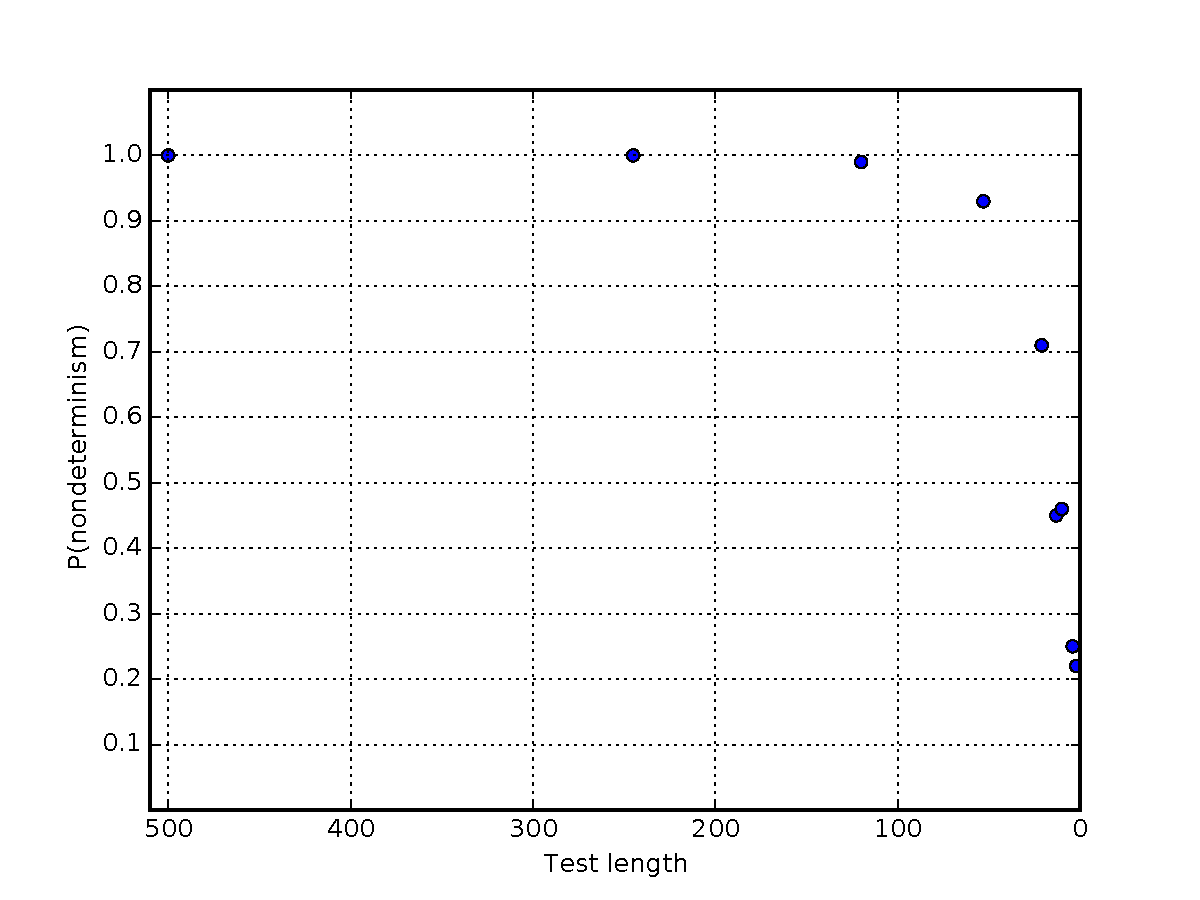
\includegraphics[width=\columnwidth]{lengthddmin}
\caption{Standard delta-debugging}
\label{fig:p1}
\end{subfigure}
\begin{subfigure}{0.67\columnwidth}
\centering
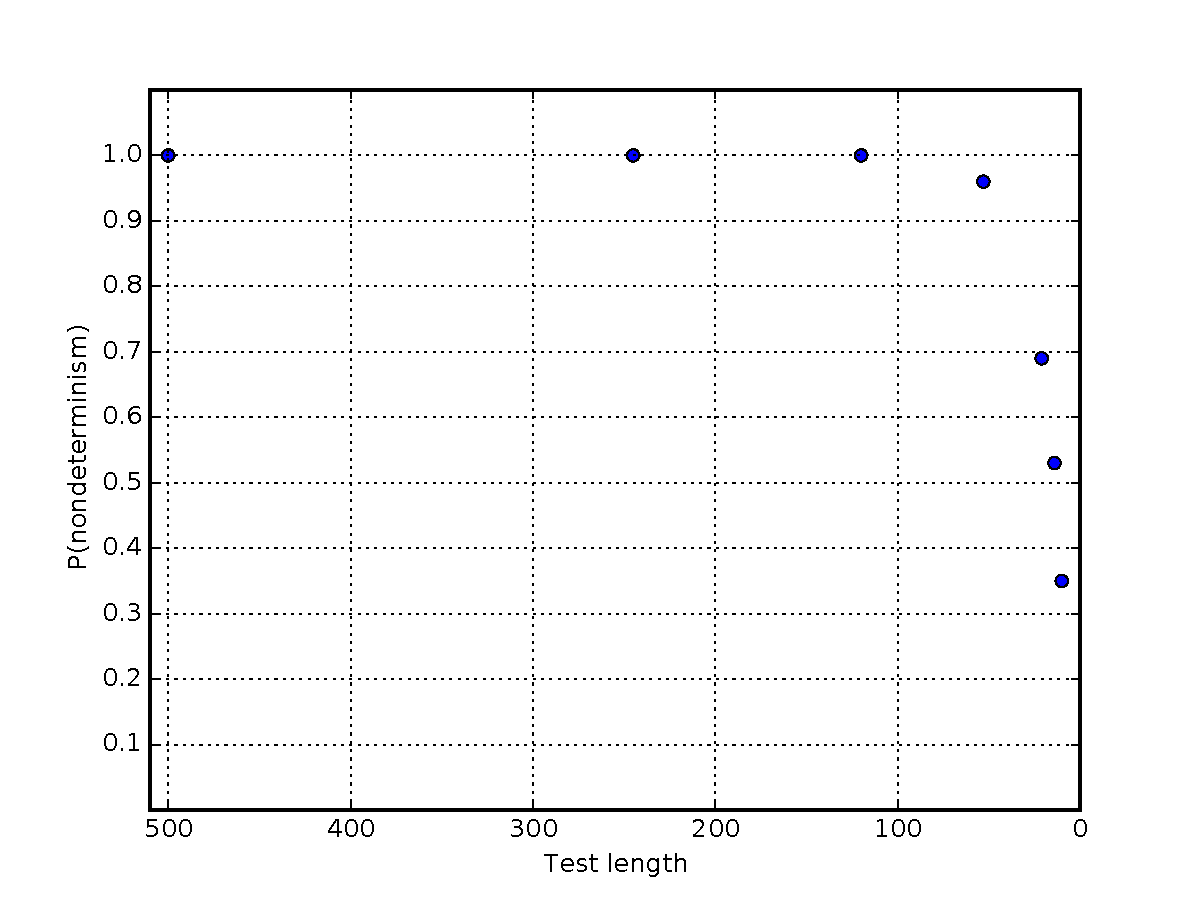
\includegraphics[width=\columnwidth]{lengthddminforcep}
\caption{P=0.5, 100 samples}
\label{fig:p2}
\end{subfigure}
\begin{subfigure}{0.67\columnwidth}
\centering
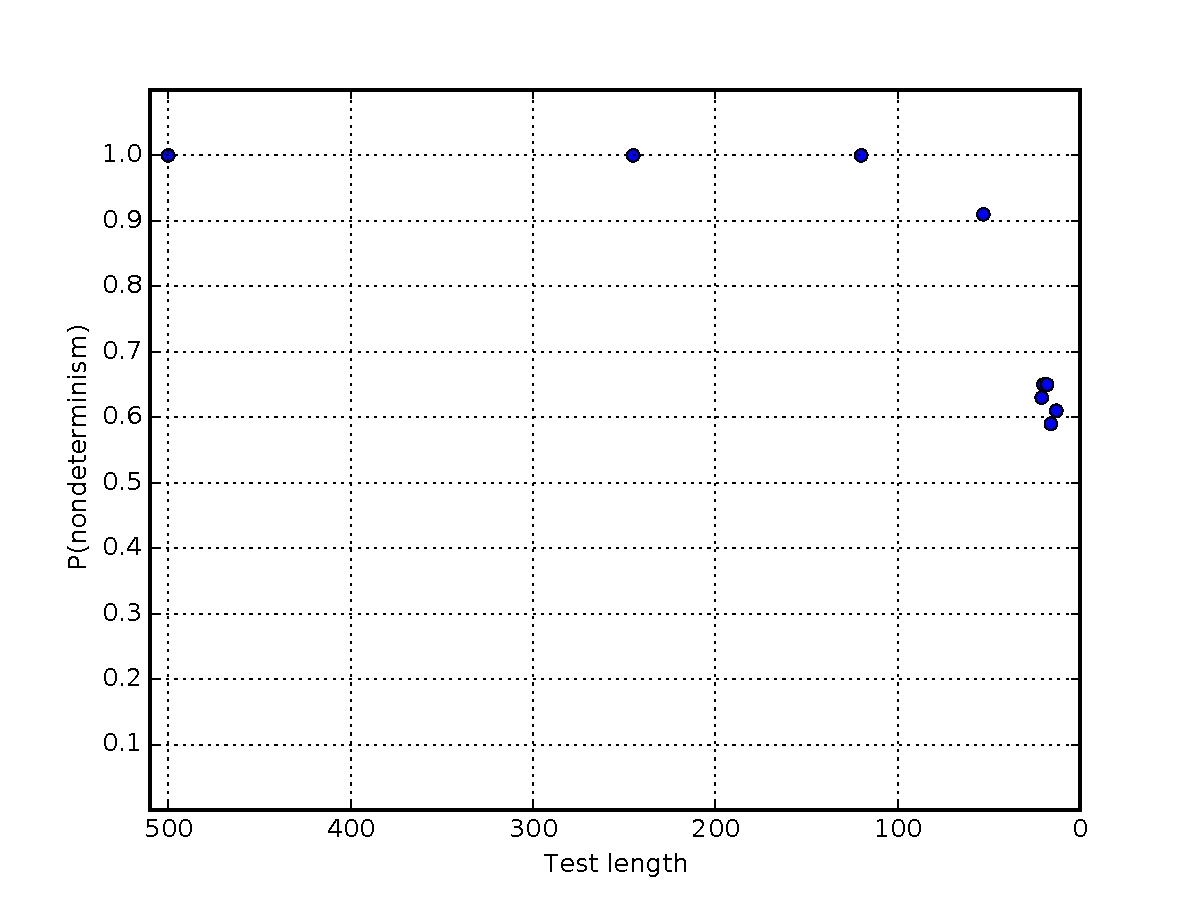
\includegraphics[width=\columnwidth]{lengthddminforceprep}
\caption{10 samples, 10 replications}
\label{fig:p3}
\end{subfigure}
\caption{Delta-debugging of the same test, with different ways of
  handling nondeterministic in the reduction predicate.}
\end{figure*}

However, simply using delta-debugging off the shelf with a predicate
like $P(fail) > 0.3 \wedge P(fail) < 1.0$, to force a test to be flaky, and force it to fail
sufficiently often to be used in debugging, will often produce
surprising and unfortunate results.  In many cases,
delta-debugging will indeed reduce the large test to a small subset.
And, in a technical sense, delta-debugging will work:  it will never
convert a nondeterministic test to a completely deterministic test,
because the reduced test that delta-debugging returns is always one
where the predicate of interest has been seen to evaluate to true.
However, if you run the resulting test, it will, in many cases, have a
$P(fail)$ that is much, much smaller than
0.3, perhaps as low as 0.01.  Why?

The problem is analogous to the problem of publication bias in
scientific fields \cite{ahmed2012assessment}.  A predicate like
$P(fail) > 0.3 \wedge P(fail) < 1.0$ cannot be evaluated by
determining the true probability of failure; rather, the test must be
run some concrete number of times, and the number of failures counted.
However, even if the number of samples $N$ is large, there is some
probability (based on the sample size) of a result that diverges
significantly from the actual probability of failure.  If the
predicate were run only once, and the number of samples reasonably
large, this would not matter.  However, by their nature,
delta-debugging and other test reduction algorithms, explore a search
space that often contains hundreds or even thousands or millions of
candidate tests.  The predicate is evaluated on each of these, and so
even with large $N$, it is extremely likely that some evaluation will
produce a very poor estimate of $P(fail)$.  If such an evaluation
causes the predicate to appear to hold for a test, delta-debugging is
``stuck'' with the error, because (to our knowledge) no test reduction
algorithms allow backtracking.  After such a mistake, finding further
reductions will become harder, but may still be possible due to the
same source of errors:  the number of experiments run is far larger
than the probability of an incorrect result.



It is the combination of
a one-way bias on faulty evaluations (the consequences of a false
positive for the predicate are much greater than for a false negative)
and the huge number of experiments relative to error rate, that
produces bad results, akin to the magnification of effect sizes
in science due to publication bias.  The bias in delta-debugging tends
towards producing a reduced test where probabilities are much smaller
than demanded by a predicate, due to the pressure on delta-debugging
to produce shorter tests.  Shorter tests have smaller probabilities,
on average, due to two factors:  first, timing-induced nondeterminism
has a much smaller temporal space to operate in (the test may be over
before a ``time-bomb'' set by an operation goes off, for example), and second, if some
test operations introduce a small probability of nondeterminism, and
only many repetitions of those operations make the probability large,
small tests obviously, on average, have fewer instances of the
problematic operations.

In scientific literature, the most frequently proposed solution is the
use of replications:  repeated runs of ``successful'' experiments to
minimize the probability that a result is a fluke due to publication
bias.  One way to produce this effect would be to allow
delta-debugging to backtrack if the probabilties observed in predicate
evaluations suddely exhibit a strong discontinuity, a kind of ``paper
retraction'' based on near-replications.  However, this requires
modifying the delta-debugging implementations, which is difficult and
sometimes not really feasible (e.g., few users of afl-fuzz \cite{aflfuzz} will wish
to change its C code for test reduction).  Ideally, the solution
should be implementable simply by modifying the predictate that is
evaluated.  

A costly but effective solution is to make $N$ large in comparison to
the number of expected predicate evaluations performed during
delta-debugging.  If the error rate is low enough, the problem
disappears.  However, given the large number of evaluations performed,
this will tend to make delta-debugging extremely slow.  We propose
using a dynamic sampling approach, where $N$ is small, but if the
predicate evaluates to true, $M$ repeated true evaluations
(``replications'', where the first true evaluation is counted as 1 replication) are
required before the predicate returns ``true'' to the delta-debugging
algorithm.  A set of $M$ repeated false positives with
$\frac{N}{M}$ samples each is much less likely than a false positive
with $N$ samples; so long as we accept the resulting bias in favor of
false negatives, we can therefore produce a reduced test with a
desired $P(fail)$ much more cheaply:  the use of replications not only
means we only pay the full sampling price on rare occasions, but a
desired accuracy for $P$ can be obtained with a much smaller value $M
\times N$ than a non-dynamically-sampled $N$.  For example, if we the predicate
is $P(fail) \geq 0.5$, and the true probability for a candidate test
is 0.25, using $N=8$ will give a false positive rate of over 10\%.
Using 4 replications on just 2 samples ($M=4;N=2$) yields a false
positive rate of about 3.7\%, yet requires almost 60\% fewer
executions of the test.  The probability calculations for such comparisons
  are relatively simple, but in real testing are
  usually not very useful, since the true
  probabilitiy distributions of test behaviors vary widely and
  dynamically during the
  delta-debugging process, making exact calculation unwieldy, even if
  the changing probabilities were known; exact results would be based on fictional
  probabilities, so gathering experimental data during a trial
  delta-debugging run and tuning $N$ and $M$ to yield desired
  results is  more effective.

Tuning $M$, any degree of confidence can be achieved, with
the basic tradeoff being between finding a test with the desired
probabilities, and the speed and effectiveness of delta-debugging.
Because increasing $M$ makes false negatives more likely, larger $M$
will usually result in less-than-optimal reduction of the original
test.



To make the basic concepts, more clear, Figures
\ref{fig:p1}-\ref{fig:p3} graphically show the interplay of
delta-debugging and nondeterministic predicates for a simple example.
In the example, tests consist of a sequence of operations that behave
nondeterministically with (independent) probabilities of 0.01, 0.05,
and 0.10, respectively, storing the value of the operation one of five array locations.
There is also an operation that clears out an array location, making
it possible to store another (possibly nondeterministic) value in that
array slot.  An example test sequence would be:

\begin{code}
array[2] = op01();
array[3] = op05();
clear(array[2]);
array[2] = op10();
\end{code}

The probability that this test behaves nondeterministically is
0.84645, the result of the simple calculation $(1-0.01) \times
(1-0.05) \times (1-0.10)$.  Figure \ref{fig:p1} shows one run of
delta-debugging on a test of length 500.  The initial test is
esentially guaranteed to behave nondeterministically; delta-debugging
only checks that it \emph{can} behave nondeterministically, and so, in
the course of reducing the test length to a test with only two
operations, the delta-debugging algorithm also reduces the probability
of nondeterminism to only about 20\%.  If we use a predicate that
``forces'' the test to behave nondeterministically at least half the
time, by sampling the predicate value 100 times and only returning
true when at least 50 of the evaluations report true, we see the
behavior in Figure \ref{fig:p2}:  the final test is slightly longer,
but still falls well short of our target of exhibiting nondeterminism
50\% of the time.  Finally, Figure \ref{fig:p3} shows what happens if
we use the same target of 50\% nondeterminism, but use only 10
samples, with 10 replications ($N$ = 10, $M$ = 10):  the test is not
much longer than in Figure \ref{fig:p2}, but the probability of
nondeterminism is above our target value, close to 60\% (and, as a bonus, fewer
test executions are required on average for each check of the predicate).  Note that
this example is purely monotonic; the pattern of probability changes
in non-monotonic settings can be even more difficult to predict and
control, but the principle of forcing a probability by sampling and
replication still holds.